\documentclass[russian,10pt,a4paper,twocolumn]{article}
\usepackage[T2A]{fontenc}
\usepackage[russian]{babel}
\usepackage[left=0cm, right=0cm, top=0cm, bottom=0cm]{geometry}
\usepackage{fancyhdr} % Для кастомных заголовков
\usepackage{graphicx} 
\usepackage{microtype}
\usepackage{microtype}

\pagestyle{fancy}

\fancyhf{}
\fancyhead[C]{\textbf{КВАНТ} $\cdot$ 1995/№ 2}  
\fancyhead[L]{24}
\renewcommand{\headrulewidth}{0pt}
\setlength{\headsep}{5pt}

\geometry{top=1cm, bottom=1cm, left=0.5cm, right=0.5cm} 

\begin{document}

	\noindent
	емой волны. Амплитуды радиосигналов, принмаемых антенной от передатчиков, одинаковы. При одновременной работе передатчиков мощность принимаемого сигнала меняется в очень широких пределах.Объясните явление и оцените суммарный процент времени, в течении которого мощность принимаего сигнала составляет менее $1/1000$ среднего значения принимаемой мощности.Отражением радиосигналов от земли пренебречь.\\
	{\slshape Р.Александров}

	\vspace{20pt}
	
	
	\noindent 
	{\LargeРешения задач М1451-1460,\\Ф1468-1477\\}
	
	
	\noindent M1451. {\slshape Даны натуральные числа $a$ и $b$ такие, что числа $\frac{a+1}{b}+\frac{b+1}{a}$ является целым. Докажите, что наибольший общий делитель чисел $a$ и $b$ не превосходит числа $\sqrt{a+b}$.}
	
	Пусть $d$ -- наибольший общий делитель чисел $a$ и $b$. \\ Так как
	\[
		\frac{a+1}{b} + \frac{b+1}{a} = \frac{a^2 +b^2 +a+b}{ab}   
	\]
	и $ab$ делится на $d^2$, то  $a^2+b^2+a+b$ делится на $d^2$.Число $a^2+b^2$ также делится на $d^2$. Поэтому $a+b$ делится на $d^2$ и $\sqrt{a+b} \ge d$\\
	{\slshape А.Голованов, Е.Малинникова}\\
	
	
	\noindent
	M1451. {\slshape Окружности $S_1$ и $S_2$ касаются внешним образом в точке $F$. Прямая $l$ касается $S_1$ и $S_2$ в точках $A$ и $B$ соответственно. Прямая параллельная прямой $l$ касается $S_2$ в точке $C$ и пересекает $S_1$ в точках $D$ и $E$. Докажите, что а) точки $A$,$F$ и $C$ лежат на одной прямой; б) общая хорда окружностей, описанных около треугольников $ABC$ и $BDE$, проходит через точку $F$. }\\
	
	\noindent
	а)Первое решение. Так как касательные к окружности $S_2$ в точках $B$ и $C$ паралельны, то $BC$ - ее диаметр, и $\angle BFC=90^{\circ}$. Проведем через точку $F$ общую касательную к окружностям(см. рисунок), пусть она пересекает прямую $l$ в точке $K$. Из равенства отрезков касательных, проведенных  к окружности из одной точки, следует, что треугольники $AKF$ и $BKF$ равнобедренные. Следовательно,
	\[
	\angle AFB=\angle AFK + \angle KFB = \angle FAB + \angle FBA = 180^{\circ}/2=90^{\circ}
	\]
	
	
\begin{figure}[h]
	\centering
	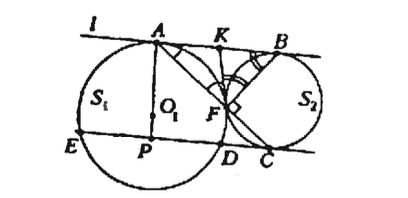
\includegraphics[width=1\linewidth]{1}
\end{figure}
	
	\noindent
	Второе решение. Рассмотрим гомотетию с центром $F$ и коэффициентом, равным $-r_1/r_2$, где $r_1$ и $r_2$ -- радиусы окружностей $S_1$ и $S_2$. При этой гомотетин $S_1$ переходит в $S_2$, а прямая $l$ -- касательная к $S_1$ -- переходит в паралельную прямую -- касательную к $S_2$. Следовательно, точка $A$ перехолдит в точку $C$, поэтому точка $F$ лежит на отрезке $AC$.\\
	б) Ниже мы покажем, что центр окружности $BDE$ находится в точке $A$. Поскольку центр окружности $ABC$ есть середина $AC$($\angle ABC=90^{\circ}$), а $\angle BFC = 90^{\circ}$(см. первое решение а)), отсюда бдет следовать, что $BF$ есть перпендекуляр, опущенный из общей точки окружностей $BDE$ и $ABC$ на прямую, соединяющую их центры. А это и значит, что прямая $BF$ содержит иъ обзую хорду.\\
	Итак, нам достаточно доказать, что $AD=AE=AB$. Первое из этих равенств очевидно (ибо касательная к $S_1$ в точке $A$ парарлельна $DE$). Пусть $r_1$ и $r_2$ - радиусы $S_1$ и $S_2$.\\ Опуская перепендекуляр $AP$ на $DE$, найдем, что\\ $AP=BC=2r_2$б и по теореме Пифагора для треугольников $APD$ и $O_1PD$, где $O_1$ -- центр $S_1$,\\
	$PD^2 = O_1D^2 - O_1p_2 = r_1^2 - (2r_2-r_1)^2=4r_1r_2-4r_2^2$,\\
	$AD^2 = AP^2 +PD^2 = 4r_1r_2$. Но легко найти, что обзая касательная $AB$ окружностей $S_1$ и $S_2$ равна $2\sqrt{r_2r_2}$.\\
	{\slshape А.Калинин, В.Дубровский} \\
	
	\noindent
	М1453.{\slshape Существует ли квадратный трехчлен $P(x)$ с целыми коэффициентами такой, что для любого натурального числа $n$, в десятичной записи коториого учавствуют одни единицы, число $P(n)$ также записывается одними единицами?}\\
	Ответ: существует.\\
	Рассмотрим квадратный трехчлен
	\[
	P(x)=x(9x+2)
	\]
	Если $n = \underbrace{11\ldots11}_k$, то $9n+2=1\underbrace{00\ldots00}_{k-1} 1$.\\
	Следовательно, $P(n)=\underbrace{11\ldots11}_k \cdot 1\underbrace{00\ldots00}_{k-1}1=\underbrace{11\cdots11}_{2k}$.\\
	Значит, этот квадратный трехчлен удовлетворяет условию.\\
	{\slshape А.Перлин}\\
	
	\noindent
	М1454.{\slshape Прямоугольник $m \times n$ разрезан на уголки:}\\
	
	\begin{figure}[h]
		\centering
		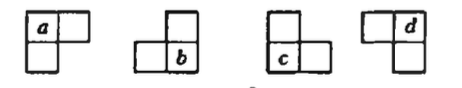
\includegraphics[width=0.8\linewidth]{2}
	\end{figure}
	
	\noindent
	{\slshape Докажите, что разность между количеством уголков вида $a$ и количеством уголоков вида $b$ делится на 3}.\\
	
	\noindent
	Ясно, что если прямоугольник $m \times n$  разрезан на уголки,то $mn$ делится на 3. Расставим в клетках прямоугольника числа так, как показано на рисунке.\\
	\renewcommand{\arraystretch}{2}
	
	\noindent
	\textls[-120]{
	\begin{tabular}{|c|c|c|c|c|c|c|c|c|}
		\hline
		1 & 2 & 3 & 4 & \ldots & n-3 & n-2 & n-1 & n \\
		\hline
		2 & 3 & 4 & 5 & \ldots & n-2 & n-1 & n & n+1 \\
		\hline
		3 & 4 & 5 & 6 & \ldots	& n-1 & n & n+1 & n+2 \\
		\hline
		\ldots & \ldots & \ldots & \ldots &  & \ldots & \ldots & \ldots & \ldots \\
		\hline
		m-1 & m & m+1 & m+2 & \ldots & m+n-5 & m+n-4 & m+n-3 & m+n-2 \\
		\hline
		m & m+1 & m+2 & m+3 & \ldots & m+n-4 & m+n-3 & m+n-2 & m+n-1 \\
		\hline
	\end{tabular}}\\

	\noindent
	Сумма всез этих чисел равна $mn(m+n)/2$. Сумма чисел, стоящих в уголке вида $a$, дает при делении на 3 остаток 2; сумма чисел, стоящих в уголке вида $b$, -- остаток 1 (или, что тоже самое, --2); суммы чисел, стоящих в уголках вида $c$ и $d$, делятся на 3. Если $n_a$ и $n_b$ -- количество уголков вида $a$ и $b$ соответственно, то сумма всех чисел в прямоугольнике имеет вид $3N+2(n_a-n_b)$, где $N$ -- некоторое число. Из равенства
	
	

	
	
\end{document}